\documentclass[12pt, letterpaper]{article}
\usepackage[margin=1 in]{geometry}
\usepackage[mathscr]{euscript}
\usepackage{amsfonts}
\usepackage{amsmath}
\usepackage{amssymb}
\usepackage{graphicx}
\usepackage{parskip}
\usepackage{minted} 
\setminted[Python]{
    frame=lines,
    framesep=2mm,
    baselinestretch=1.2,
    bgcolor=LightGray
}
\usepackage{xcolor} % to access the named colour LightGray
\definecolor{LightGray}{gray}{0.9}
\usepackage{listings}% http://ctan.org/pkg/listings
\lstset{
  basicstyle=\ttfamily,
  mathescape
}
\graphicspath{{./images/}}
\setlength{\parindent}{0pt}
\newcommand{\R}{\mathbb{R}}
\newcommand{\mdash}{
\draw(0.3,0.5ex)--(-0.3,0.5ex);
}

\title{Deep Learning Specialization}
\author{Declan Lim}

\begin{document}>
    \maketitle
    \pagebreak

    \section{Neural Networks and Deep Learning}
    \subsection{Introduction to Deep Learning}
    \begin{itemize}
        \item Takes input $x$ to a ``neuron'' and gives some output $y$   
        \begin{figure}[ht]
            \centering
            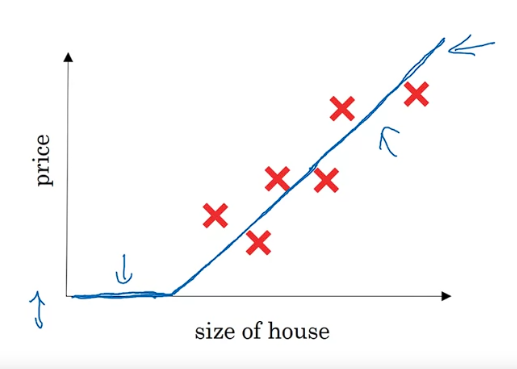
\includegraphics[width=8cm]{1.png}
        \end{figure}
        \begin{itemize}
            \item Simple neural network has a single input, neuron and output
            \item $x$: size of the house
            \item $y$: price of the house
            \item Hypothesis (blue line) is a ReLU (Rectified Linear Unit)
        \end{itemize}
        \item More complex neural networks can be formed by ``stacking'' neurons
        \begin{figure}[ht]
            \centering
            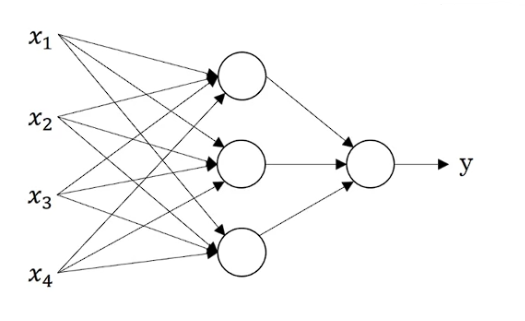
\includegraphics[width=8cm]{2.png}
        \end{figure}
        \item Every input layer feature is interconnected with every hidden layer feature
        \begin{itemize}
            \item The neural network will decide what the intermediate features will be
        \end{itemize}
        \item Most useful in supervised learning settings
    \end{itemize}
    \hspace{3mm}
    \subsubsection{Supervised Learning}
    \begin{itemize}
        \item Aims to learn a function to map an input $x$ to an output $y$
        \begin{itemize}
            \item Real estate: predicting house prices from the house features
            \item Online advertising: showing ads based on probability of user clicking on ad
            \item Photo tagging: tagging images based on objects in the image
            \item Speech recognition: generating a text transcript from audio
            \item Machine translation: translating from one language to another
            \item Autonomous driving: returning the positions of other cars from images and radar info
        \end{itemize}
        \item Different types of neural network used for different tasks
        \begin{itemize}
            \item Standard neural network: real estate and online advertising
            \item Convolutional neural network (CNN): image data
            \item Recurrent neural network (RNN): audio and language data (sequenced data)
            \item Hybrid neural network: Autonomous driving (more complex input)
        \end{itemize}
        \begin{figure}[ht]
            \centering
            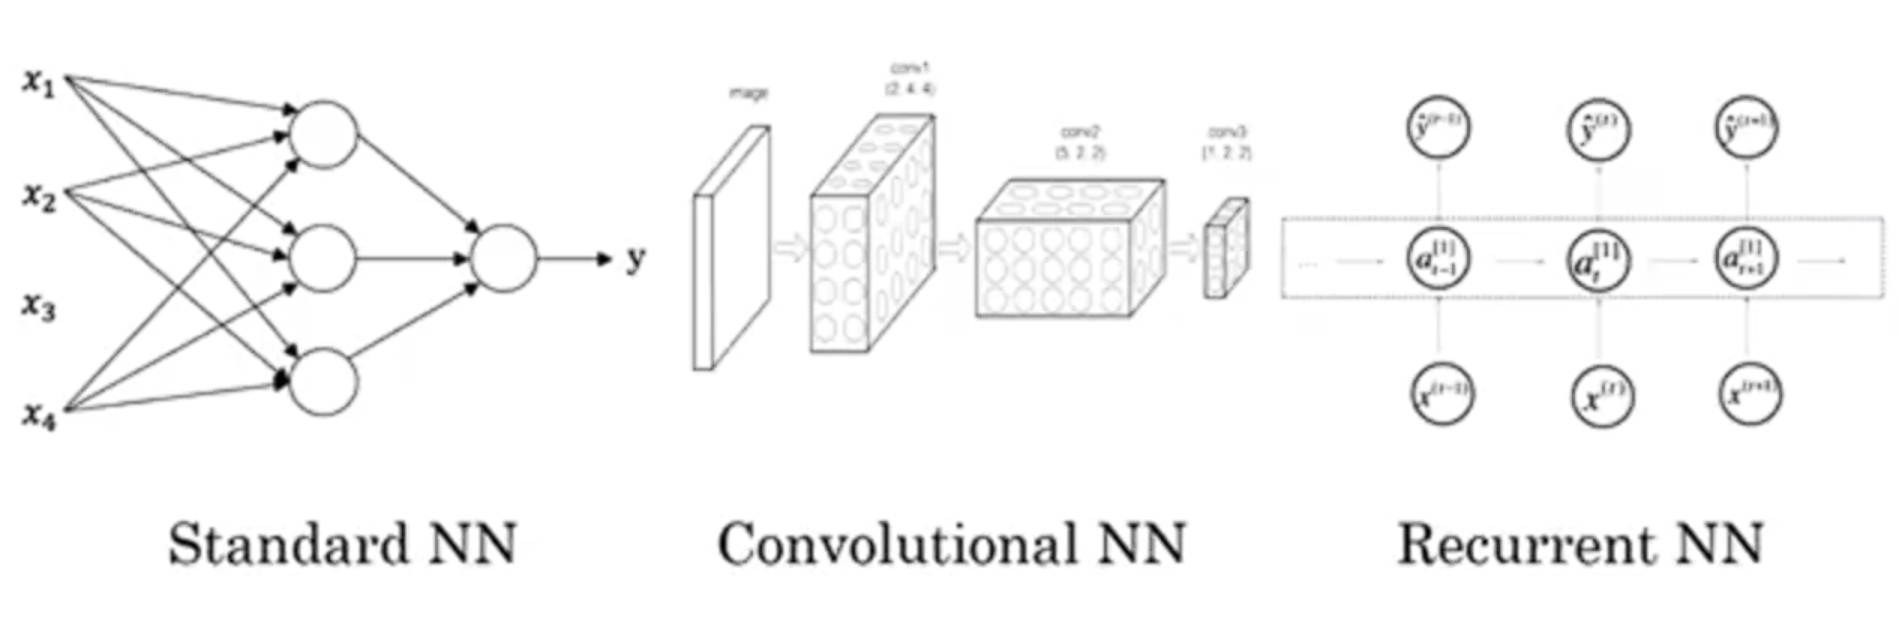
\includegraphics[width=10cm]{3.png}
        \end{figure}
        \item Supervised learning can be applied to structured and unstructured data
        \begin{itemize}
            \item Structured data has features with well defined meanings 
            \item Unstructured data has more abstract features (images, audio, text)
        \end{itemize}
    \end{itemize}

    \hspace{30mm}
    \begin{itemize}
        \item Deep learning has only recently started to become more widespread
        \begin{itemize}
            \item Given large amounts of data and a large NN, deep learning will outperform more traditional learning algorithms
            \item For small amounts of data, any performance of the algorithm depends on specific implementation
        \end{itemize}
        \begin{figure}[ht]
            \centering
            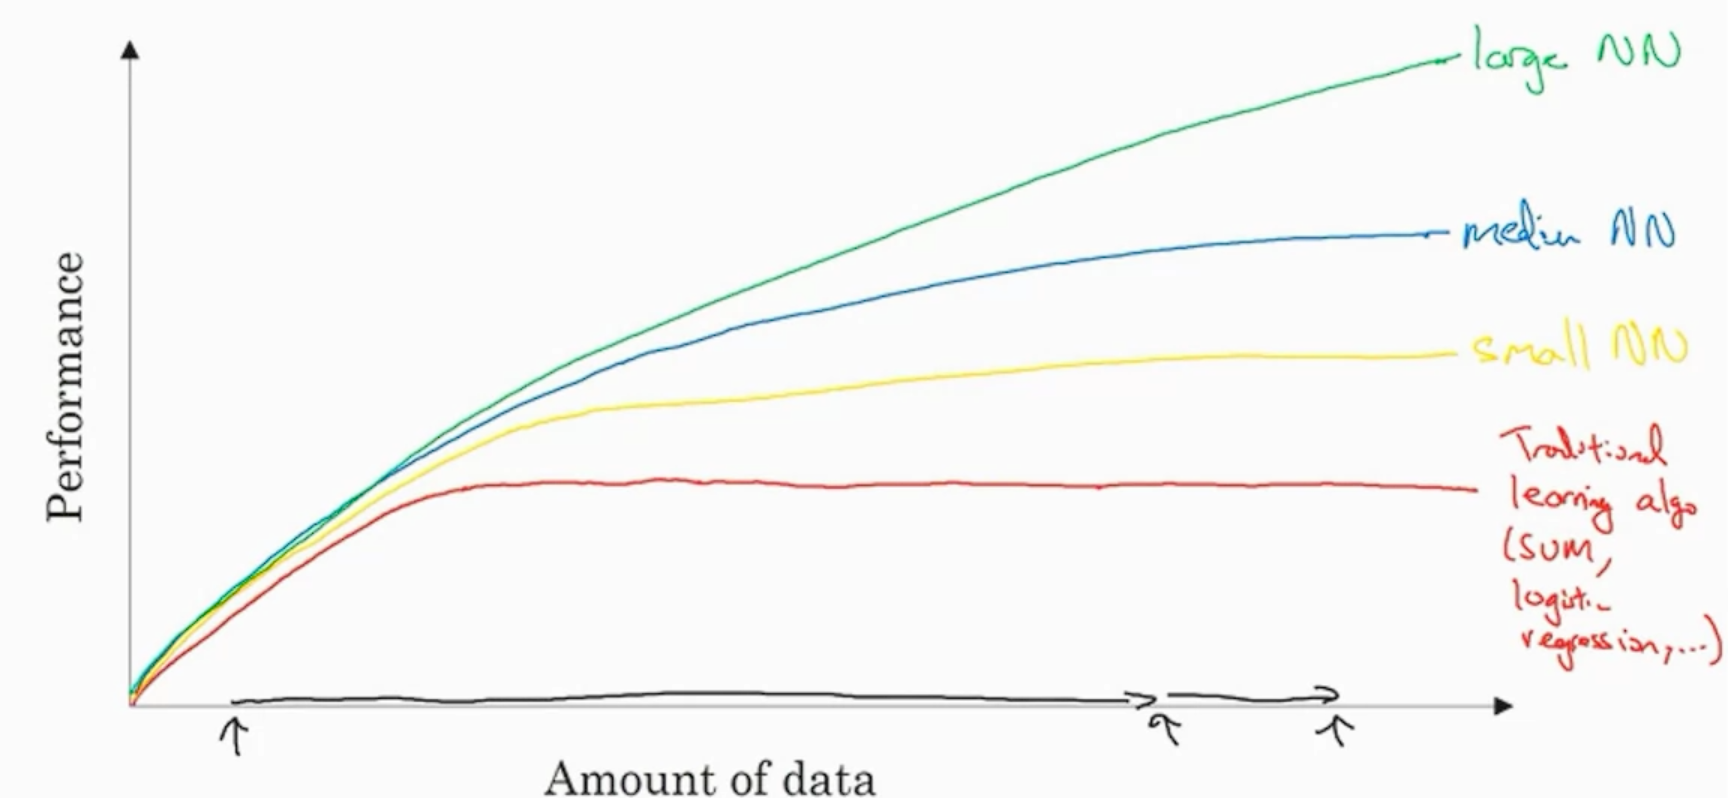
\includegraphics[width=8cm]{4.png}
        \end{figure}
        \item ``Scale drives deep learning progress''
        \begin{itemize}
            \item Both the scale of the data and the NN
        \end{itemize}
        \item Recent algorithmic innovations with increase scale of computation
        \begin{itemize}
            \item Idea to switch from sigmoid activation function to ReLu function increased NN performance
            \item Ends of sigmoid function have close to 0 gradient so and therefore result in small changes in $\theta$
            \item ReLu function has gradient of 1 for positive values
        \end{itemize}
        \item Neural network process is iterative
        \begin{itemize}
            \item Increasing speed at which a NN can be trained allows different ideas to be tried
        \end{itemize}
    \end{itemize}
    \subsection{Neural Network Basics}
    \subsubsection{Logistic Regression as a Neural Network}
    \begin{itemize}
        \item Logistic regression used for binary classification
        \item For a colour image, of 64$\times$64 pixels, will have total 12288 input features
        \begin{itemize}
            \item Image is stored as 3 separate matrices for each colour channel
            \item All pixel intensities should be unrolled into a single feature vector
            $$n=12288$$
            $$x\in\R^{12288}$$
            \item For a matrix \texttt{X} of shape $(a,b,c,d)$, want a matrix \texttt{X\_flatten} of shape $(b*c*d,1)$
        \end{itemize}
        \begin{minted}{Python}
            X_flatten = X.reshape(X.shape[0], -1).T
        \end{minted}
        
    \end{itemize}
    
    \vspace{5mm}
    \textbf{Notation} 
    $$\{(x^{(1)},y^{(1)}),(x^{(2)},y^{(2)}),...,(x^{(m)},y^{(m)})\}$$
    \begin{itemize}
        \item $(x,y)$: single training example
        \begin{itemize}
            \item $x\in\R^{n_x}$ ($n_x=$ number of features)
            \item $y\in\{0,1\}$
        \end{itemize}
        \item $(x^{(i)},y^{(i)})$: $i^{th}$ training example
        \item $m=m_{train}$
        \item $m_{test}=$ \# of test examples
        \item $X=\begin{bmatrix}
            \mid & \mid & & \mid \\
            x^{(1)} & x^{(2)} & ... & x^{(3)} \\
            \mid & \mid & & \mid \\
        \end{bmatrix}$
        \begin{itemize}
            \item $X\in\R^{n_x\times n}$
        \end{itemize}
        \item $Y=\begin{bmatrix}
            y^{(1)} & y^{(2)} & ... & y^{(m)}
        \end{bmatrix}$
        \begin{itemize}
            \item $Y\in\R^{1\times m}$
        \end{itemize}
    \end{itemize}

    \vspace{5mm}
    \textbf{Logistic Regression}
    \begin{itemize}
        \item Given $x$, want $\hat{y}=P(y=1|x)$
        \begin{itemize}
            \item Since $\hat{y}$ is a probability, want $0\leq\hat{y}\leq1$
        \end{itemize}
        \item Parameters: $w\in\R^{n_x}, b\in\R$
        \item Output: $\hat{y}=\sigma(w^Tx+b)$
        \begin{figure}[ht]
            \centering
            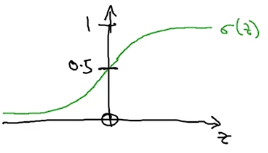
\includegraphics[width=8cm]{5.png}
        \end{figure}
        $$\sigma(z)=\frac{1}{1+e^{-z}}$$
        $$z=w^Tx+b$$
        \item Aim is to learn parameters $w$ and $b$ such that $\hat{y}$ is a good estimate of the probability
        \item Previous convention had $\theta$ vector with an additional $\theta_0$ parameter
        \begin{itemize}
            \item Keeping $\theta_0$ ($b$) separate from the rest of the parameters is easier to implement
        \end{itemize}
    \end{itemize}

    \vspace{3mm}
    \textbf{\textit{Cost Function}}
    \begin{itemize}
        \item Given $\{(x^{(1)}, y^{(1)}),(x^{(2)}, y^{(2)}), ..., (x^{(m)}, y^{(m)})\}$, want $\hat{y}^{(i)} \approx y^{(i)}$
        \item Squared error function not used for logistic regression loss function 
        \begin{itemize}
            \item Optimization problem becomes non convex and will have local optima
        \end{itemize}

        \vspace{10mm}
        $$\mathcal{L}(\hat{y},y)=-(y\log(\hat{y})+(1-y)\log(1-\hat{y}))$$
        \item If $y=1$:
        \begin{itemize}
            \item $\mathcal{L}(\hat{y},y)=-\log(\hat{y})$
            \item Want large $\log(\hat{y})$ $\therefore$ want large $\hat{y}$
            \item $\hat{y}$ has a max of 1 $\therefore$ want $\hat{y}=1$
        \end{itemize}
        \item If $y=0$:
        \begin{itemize}
            \item $\mathcal{L}(\hat{y}, y)=-log(1-\hat{y})$
            \item Want large $\log(1-\hat{y})$ $\therefore$ want small $\hat{y}$
            \item $\hat{y}$ has a min of 0 $\therefore$ want $\hat{y}=0$
        \end{itemize}
        \item Cost function:
        \begin{align*}
            J(w,b)&=\frac{1}{m}\sum_{i=1}^{m}\mathcal{L}(\hat{y}^{(i)},y^{(i)}) \\
            &= -\frac{1}{m}\sum_{i=1}^{m}[y^{(i)}\log(\hat{y}^{(i)})+(1-y^{(i)})\log(1-\hat{y}^{(i)})]
        \end{align*}
        \begin{itemize}
            \item Average loss function over all training examples
        \end{itemize}
    \end{itemize}

    \vspace{3mm}
    \textbf{\textit{Gradient Descent}}
    \begin{itemize}
        \item Want to find values of $w$ and $b$ that minimize the cost function $J(w,b)$
        \begin{itemize}
            \item For logistic regression, $w$ and $b$ usually initialized to 0
        \end{itemize} 
        \item One iteration of gradient descent will take a step in the direction of steepest descent
    \end{itemize}

    \vspace{3mm}
    \begin{lstlisting}
    Repeat {
        w := w - $\alpha \frac{\partial J(w,b)}{\partial w}$
        b := b - $\alpha \frac{\partial J(w,b)}{\partial b}$
    }  
    \end{lstlisting}
    \begin{itemize}
        \item Using the computation graph:
        \begin{figure}[ht]
            \centering
            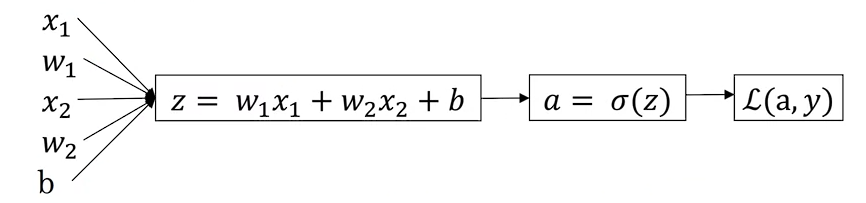
\includegraphics[width=12cm]{6.png}
        \end{figure}
        \begin{center}
            $$\frac{\partial \mathcal{L}(a,y)}{\partial a}=-\frac{y}{a}+\frac{1-y}{1-a}$$
            \begin{align*}
                \frac{\partial\mathcal{L}(a,y)}{\partial z} &=\frac{\partial\mathcal{L}}{\partial a} \times \frac{\partial a}{\partial z} \\
                &= (-\frac{y}{a}+\frac{1-y}{1-a}) \times a(1-a) \\
                &= a-y
            \end{align*}
            $$\frac{\partial\mathcal{L}}{\partial w_1}=x_1 \times \frac{\partial\mathcal{L}}{\partial z}$$
            $$\frac{\partial\mathcal{L}}{\partial w_2}=x_2 \times \frac{\partial\mathcal{L}}{\partial z}$$
            $$\frac{\partial\mathcal{L}}{\partial b}=\frac{\partial\mathcal{L}}{\partial z}$$
        \end{center}
        \item Partial derivative over all training examples calculated by taking the average \texttt{dw1}
        $$\frac{\partial}{\partial w_1}J(w,b)=\frac{1}{m}\sum^m_{i=1}\frac{\partial}{\partial w_1} \mathcal{L}(a^{(i)},y^{(i)})$$

        Initialize \texttt{J = 0, dw1 = 0, dw2 = 0, db = 0}
        \begin{lstlisting}
        For i = 1 to m:
            z$^{(i)}$ = w$^T$x$^{(i)}$ + b
            a$^{(i)}$ = $\sigma$(z$^{(i)}$)

            J += -[y$^{(i)}$ $\log$(a$^{(i)}$) + (1-y$^{(i)}$)$\log$(1-a$^{(i)}$)]
            dz$^{(i)}$ = a$^{(i)}$ - y$^{(i)}$
            dw1 += x$_1^{(i)}$ dz$^{(i)}$
            dw2 += x$_2^{(i)}$ dz$^{(i)}$
            db += dz$^{(i)}$

        J /= m
        dw1 /= m
        dw2 /= m
        db /= m

        w1 := w1 - $\alpha$ dw1
        w2 := w2 - $\alpha$ dw2 
        b := b - $\alpha$ db
        \end{lstlisting}
        \item Above implementation requires \texttt{for} loop over all features for all training examples
        \begin{itemize}
            \item Vectorization can be used to remove explicit \texttt{for} loops
            \item Vectorization required for deep learning to be efficient
        \end{itemize}
    \end{itemize}

    \subsubsection{Vectorisation in Python}
    \begin{itemize}
        \item Deep learning performs best on large data sets
        \begin{itemize}
            \item Code must be able to run quickly to be effective on large data sets
        \end{itemize}
        $$z=w^Tx + b$$
        $$w\in \R^{n_x} ~~ x\in \R^{n_x}$$
        \item Non vectorized implementation:
        \begin{minted}{Python}
            z = 0
            for i in range(n_x):
                z += w[i] * x[i]
            z += b
        \end{minted}
        \item GPUs and CPUs both have parallelization instructions (SIMD: Single Instruction Multiple Data)
        \begin{itemize}
            \item If built in functions are used, \texttt{numpy} will use parallelism to perform computations faster 
        \end{itemize}
        \item For logistic regression, need to calculate $z$ and $a$ values for each training example
        $$z^{(i)}=w^Tx^{(i)}+b$$
        $$a^{(i)}=\sigma(z^{(i)})$$
        $$X = \begin{bmatrix}
            \mid & \mid & & \mid \\
            x^{(1)} & x^{(2)} & ... & x^{(m)} \\
            \mid & \mid & & \mid 
        \end{bmatrix} $$
        $$w\in\R^{n_x} ~~ X\in\R^{n_x\times m}$$ 
        \begin{align*}
            \begin{bmatrix}
                z^{(1)} & z^{(2)} & ... & z^{(m)}
            \end{bmatrix}
            &= w^TX + \begin{bmatrix}
                b & b & ... & b
            \end{bmatrix} \\
            &= \begin{bmatrix}
                w^Tx^{(1)}+b & w^Tx^{(2)}+b & ... & w^Tx^{(m)}+b 
            \end{bmatrix}
        \end{align*}
        \item In Python:
        \begin{minted}{Python}
            Z = np.dot(w.T, X) + b
        \end{minted}
        \begin{itemize}
            \item Python will broadcast the value \texttt{b} so it can be added to the matrix
        \end{itemize}
        \item Vectorized implementation of sigmoid function can be used on \texttt{Z} to calculate \texttt{A}
        $$A= \begin{bmatrix}
            a^{(1)} & a^{(2)} & ... & a^{(m)}
        \end{bmatrix} $$
        
        $$dz^{(i)}=a^{(i)}-y^{(i)}$$
        $$dz=A-Y$$
        $$db=\frac{1}{m}\sum^m_{i=1}dz^{(i)}$$
        $$dw=\frac{1}{m}X(dz)^T$$
        \begin{minted}{Python}
            Z = np.dot(w.T,X) + b
            A = sigmoid(Z)
            dz = A - Y
            dw = 1/m * np.dot(X, dz.T)
            db = 1/m * np.sum(dz)

            # Gradient descent update
            w = w - alpha * dw
            b = b - alpha * db
        \end{minted}
        \item \texttt{for} loop is required to run multiple iterations of gradient descent
    \end{itemize}
    \subsection{Shallow Neural Networks}
    \begin{itemize}
        \item A neural network will have stacked logistic regression units in each layer
        \begin{itemize}
            \item Logistic regression output from one layer will be fed to another layer
        \end{itemize}
    \end{itemize}

    \vspace{25mm}
    \begin{itemize}
        \begin{figure}[ht]
            \centering
            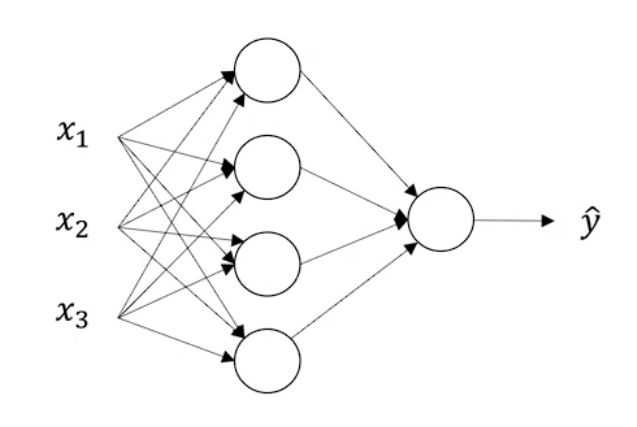
\includegraphics[width=8cm]{7.png}
        \end{figure}
        \item Input layer of the neural network contains the feature $x_1, x_2, x_3$
        \begin{itemize}
            \item $a^{[0]}=X$    
        \end{itemize}
        \item Intermediate layers in the network are hidden layers
        \begin{itemize}
            \item Hidden layers do not have ``true'' values in the training set
        \end{itemize}
        \item Final layer in the network is the output layer
        \begin{itemize}
            \item Generates the predicted value $\hat{y}$
        \end{itemize}
        \item Above diagram is a 2 layer NN
        \begin{itemize}
            \item Input layer is layer 0
        \end{itemize}
        \item Each layer will have parameters $w$ and $b$ associated with them 
        \item Each node in the NN will perform logistic regression with its inputs
        $$z_i^{[l]}=w_i^{[l]T}x+b_i^{[l]} ~~\rightarrow~~ a_i^{[l]}=\sigma(z_i^{[l]})$$
      

        $$W^{[1]} = \begin{bmatrix}
            - & w_1^{[1]T} & - \\
            - & w_2^{[1]T} & - \\
            - & w_3^{[1]T} & - \\
            - & w_4^{[1]T} & - 
        \end{bmatrix} $$
        $$a^{[0]}=\begin{bmatrix}
            x_1 \\
            x_2 \\
            x_3
        \end{bmatrix} $$
        $$b^{[1]}=\begin{bmatrix}
            b_1^{[1]} \\
            b_2^{[1]} \\
            b_3^{[1]} \\
            b_4^{[1]} 
        \end{bmatrix}$$

        \begin{align*}
            z^{[1]}&=\begin{bmatrix}
                z_1^{[1]} \\
                z_2^{[1]} \\
                z_3^{[1]} \\
                z_4^{[1]} \\
            \end{bmatrix} \\
            &= \begin{bmatrix}
                w_1^{[1]T}a^{[0]}+b_1^{[1]} \\
                w_2^{[1]T}a^{[0]}+b_1^{[1]} \\
                w_3^{[1]T}a^{[0]}+b_1^{[1]} \\
                w_4^{[1]T}a^{[0]}+b_1^{[1]} \\
            \end{bmatrix} \\
            &= w^{[1]} a^{[0]} + b^{[1]}
        \end{align*}

        \begin{align*}
            a^{[1]}&=\begin{bmatrix}
                a_1^{[1]} \\
                a_2^{[1]} \\
                a_3^{[1]} \\
                a_4^{[1]} \\
            \end{bmatrix} \\
            &= \sigma(z^{[1]})
        \end{align*}
        $$z^{[2]}=W^{[2]}a^{[1]}+b^{[2]} ~~\rightarrow~~ a^{[2]}=\sigma(z^{[2]})$$
    \end{itemize}

    \begin{itemize}
        \item Vectorized method should be able to work on all training examples at one time
        \begin{itemize}
            \item Vector for each training example can be stacked horizontally in a matrix
            \item Vertical dimension will be the number of units in a layer ($n_x$ for the input layer)
        \end{itemize}
    \end{itemize}

    $$X=\begin{bmatrix}
        \mid & \mid & & \mid \\
        x^{(1)} & x^{(2)} & & x^{(m)} \\
        \mid & \mid & & \mid
    \end{bmatrix}$$

    $$Z^{[1]}=\begin{bmatrix}
        \mid & \mid & & \mid \\
        z^{[1](1)} & z^{[1](2)} & ... & z^{[1](m)} \\
        \mid & \mid & & \mid
    \end{bmatrix}$$

    $$A^{[1]}=\begin{bmatrix}
        \mid & \mid & & \mid \\
        a^{[1](1)} & a^{[1](2)} & ... & a^{[1](m)} \\
        \mid & \mid & & \mid
    \end{bmatrix}$$
    
    \begin{align*}
        Z^{[1]}&=W^{[1]}X+b^{[1]} \\
        A^{[1]}&=\sigma(Z^{[1]}) \\
        Z^{[2]}&=W^{[2]}A^{[1]}+b^{[2]} \\
        A^{[2]}&=\sigma(Z^{[2]})
    \end{align*}

    \subsubsection{Activation Functions}
    \begin{itemize}
        \item After $z$ values are calculated, activation function must be run to get the activation value $a$
        $$a_{sigmoid}=\frac{1}{1+e^{-z}}$$
        \item Alternatively $a^{[1]}=g(z^{[1]})$ where $g$ is a non linear function
        \item $\tanh$ function almost always performs better than the sigmoid function
        \begin{itemize}
            \item Equivalent to a transformed version of the sigmoid function  
            \item $\tanh$ function is odd and is ``centered'' around the origin
            \item The mean of the data will be closer to 0 and will help with learning in the next layer
        \end{itemize}
        $$a_{\tanh}=\frac{e^z-e^{-z}}{e^z+e^{-z}}$$
        \begin{figure}[ht]
            \centering
            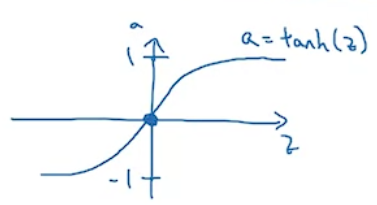
\includegraphics[width=8cm]{8.png}
        \end{figure}
        \item For binary classification, the final output layer can use the sigmoid function
        \begin{itemize}
            \item Want the value of $\hat{y}$ to be between 0 and 1
        \end{itemize}
        \item For both the sigmoid and $\tanh$ functions, when $z$ is large, the gradient is very small
        \begin{itemize}
            \item Results in a slower gradient descent
        \end{itemize}
        \item ReLU function has a gradient of 1 when $z$ is positive
        \begin{figure}[ht]
            \centering
            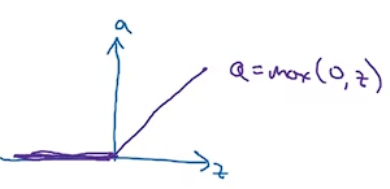
\includegraphics[width=8cm]{9.png}
        \end{figure}
        \begin{itemize}
            \item Gradient is 0 when $z$ is negative
        \end{itemize}
        \item For majority of the ReLU function, gradient is very different from 0
        \begin{itemize}
            \item Will typically allow NN to learn much faster than sigmoid or $\tanh$ function
        \end{itemize}
        \item ReLU function should be used as the default activation function
        \item The leaky ReLu function has a slight positive gradient when $z$ is negative
        $$a_{leaky ReLU}=\max(0.01z, z)$$
        \begin{figure}[ht]
            \centering
            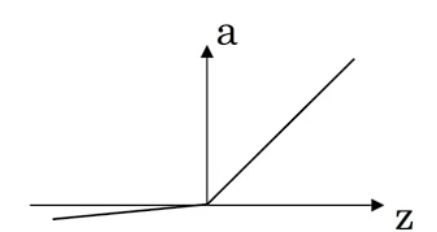
\includegraphics[width=8cm]{10.png}
        \end{figure}
        \item For a NN to compute more complex functions, activation function must be non linear
        \begin{itemize}
            \item If a linear activation function is used, final output of the NN can only be a linear function 
            \item Multiple linear activation neurons with a sigmoid as the output neuron is equivalent to standard logistic regression
        \end{itemize}
        \item Linear activation function can be used in the output layer if output is a real number
        \item Derivative of the activation function must be calculated for backpropagation
        \begin{itemize}
            \item Sigmoid function
            $$g(z)=\frac{1}{1+e^{-z}}$$
            \begin{align*}
                \frac{d}{dz}g(z)&=\frac{1}{1+e^{-z}}\left(1-\frac{1}{1+e^{-z}}\right) \\
                &=g(z)(1-g(z))
            \end{align*}
            \item $\tanh$ function
            \begin{align*}
            g(z)&=\tanh(z) \\
            &=\frac{e^z-e^{-z}}{e^z+e^{-z}}
            \end{align*}
            \begin{align*}
                \frac{d}{dz}g(z)&=1-\left(\frac{e^z-e^{-z}}{e^z+e^{-z}}\right)^2 \\
                &=1-g(z)^2
            \end{align*}
            \item ReLU function
            $$g(z)=\max(0,z)$$
            $$\frac{d}{dz}g(z)=\begin{cases}
                0 & \text{if } z < 0 \\
                1 & \text{if } z \geq 0
            \end{cases}$$
            \item Leaky ReLU function
            $$g(z)=\max(0.01z,z)$$
            $$\frac{d}{dz}g(z)=\begin{cases}
                0.01 & \text{if } z < 0 \\
                1 & \text{if } z \geq 0
            \end{cases}$$
        \end{itemize}

    \end{itemize}
    \subsubsection{Gradient Descent for Neural Networks}
    \begin{itemize}
        \item For a single hidden layer NN, parameters are: $w^{[1]}, b^{[1]}, w^{[2]}, b^{[2]}$
        \begin{itemize}
            \item $w^{[1]}\in\R^{n_1\times n_0}$
            \item $b^{[1]}\in\R^{n_1\times 1}$
            \item $w^{[2]}\in\R^{n_2\times n_1}$
            \item $b^{[2]}\in\R^{n_2\times 1}$
        \end{itemize}
        \item Cost function: $J(w^{[1]}, b^{[1]}, w^{[2]}, b^{[2]})=\frac{1}{m}\sum_{i=1}^n\mathcal{L}(\hat{y},y)$
        \item For one iteration of gradient descent:
        $$w^{[1]}:=w^{[1]}-\alpha dw^{[1]},~b^{[1]}:=b^{[1]}-\alpha db^{[1]}$$
        $$w^{[2]}:=w^{[2]}-\alpha dw^{[2]},~b^{[2]}:=b^{[2]}-\alpha db^{[2]}$$
        \begin{itemize}
            \item Gradient descent step will take place after backpropagation calculates the derivatives
        \end{itemize}
        \item Forward propagation:
        \begin{align*}
            Z^{[1]}&=W^{[1]}X+b^{[1]} \\
            A^{[1]}&=g^{[1]}(Z^{[1]}) \\
            Z^{[2]}&=W^{[2]}A^{[1]}+b^{[2]} \\
            A^{[2]}&=g^{[2]}(Z^{[2]})
        \end{align*}
        \item Backpropagation:
        \begin{align*}
            dz^{[2]}&=A^{[2]}-Y \\
            dw^{[2]}&=\frac{1}{m}dz^{[2]}A^{[1]T} \\
            db^{[2]}&=\frac{1}{m}\texttt{np.sum}(dz^{[2]}, \texttt{axis = 1, keepdims = True}) \\
            dz^{[1]}&=w^{[2]T}dz^{[2]}\times g^{[1]'}(z^{[1]}) \\
            dw^{[1]}&=\frac{1}{m}dz^{[1]}X^T \\
            db^{[1]}&=\frac{1}{m}\texttt{np.sum}(dz^{[1]}, \texttt{axis = 1, keepdims = True})
        \end{align*}
    \end{itemize} 

    \subsubsection{Random Initialization}
    \begin{itemize}
        \item Weights must be initialized randomly for a NN
        \begin{itemize}
            \item Weights can be initialized to 0 for logistic regression
            \item The bias terms $b$ can be initialized
        \end{itemize}
        \item If weights are initialized to 0, all neurons in a layer will compute the same hypothesis
        \begin{minted}{Python}
            W1 = np.random.randn((2,2)) * 0.01
            b1 = np.zero((2,1))  
        \end{minted}
        \item Weights should be initialized to small random values
        \begin{itemize}
            \item If weight is too large, activation value $z^{[1]}$ will be large
            \item If sigmoid or $\tanh$ function is used, derivative will be very small and learning will be very slow
        \end{itemize}
        \item Different constant for \texttt{np.random.randn} should be used for deeper neural networks
    \end{itemize}
    \subsection{Deep Neural Networks}
    \begin{itemize}
        \item Logistic regression is equivalent to a 1-layer NN
        \item Deep NN have more hidden layers
        \begin{itemize}
            \item Number of hidden layers in the network can be a parameter for the ML problem
        \end{itemize}
        
        \vspace{25mm}
        \begin{figure}[ht]
            \centering
            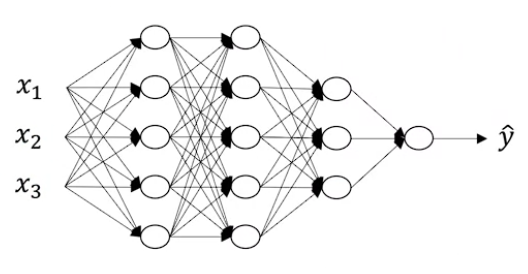
\includegraphics[width=8cm]{11.png}
        \end{figure}
        \begin{itemize}
            \item Above network has 4 layers, $L=4$
            \item $n^{[l]}=$ number of units in layer $l$
            \item $a^{[l]}=$ activations in layer $l$
        \end{itemize}
        \item The inputs $x$ are the activations of the first layer, $x=a^{[0]}$
        \begin{itemize}
            \item Prediction $\hat{y}$ will be the activations of the last layer, $\hat{y}=a^{[L]}$
        \end{itemize}
        \item Forward propagation for a deep NN will follow the same pattern for all layers
        $$z^{[l]}=w^{[l]}a^{[l-1]}+b^{[l]}$$
        $$a^{[l]}=g^{[l]}(z^{[l]})$$
        \item For a vectorized implementation
        $$Z^{[l]}=W^{[l]}A^{[l-1]}+b^{[l]}$$
        $$A^{[l]}=g^{[l]}(z^{[l]})$$
        \begin{itemize}
            \item Explicit for loop will be used to loop over the layers in the network
            \item $b$ will still be a column vector but will apply correctly due to broadcasting
            \item When working with $W$ and $A$ matrices, $A$ will be for the previous layer so the dimensions will fit
        \end{itemize}
        \item When debugging NN, can look at dimensions of all the matrices
        \item For a non vectorized implementation:
        \begin{itemize}
            \item $W^{[l]}:(n^{[l]},n^{[l-1]})$
            \item $b^{[l]}:(n^{[l]},1)$
            \item Dimensions of $dw$ and $db$ should be the same as the dimensions of $W$ and $b$
            \item $a^{[l]}, z^{[l]}:(n^{[l]},1)$ 
        \end{itemize}
        \item For a vectorized implementation, $z$ vectors and $a$ vectors will be stacked horizontally for all training examples
        \begin{itemize}
            \item $Z^{[l]},A^{[l]}:(n^{[l]},m)$
        \end{itemize}
        \item Deep NN tend to work better as each layer can compute increasingly complex functions
        \begin{itemize}
            \item Face recognition: edge detection $\rightarrow$ individual features $\rightarrow$ large parts of the face
            \item Audio: low level waveforms $\rightarrow$ phonemes $\rightarrow$ words $\rightarrow$ sentences
        \end{itemize}
        \item Functions that can be computed with a ``small'' deep neural network require exponentially more hidden units in a shallower network
        \item For each forward propagation step, the value of $z^{[l]}$ should be cached for backpropagation
        \begin{itemize}
            \item Values of $w^{[l]}$ and $b^{[l]}$ can also be stored in the cache so they can be accessed for backpropagation
        \end{itemize}
        \begin{figure}[ht]
            \centering
            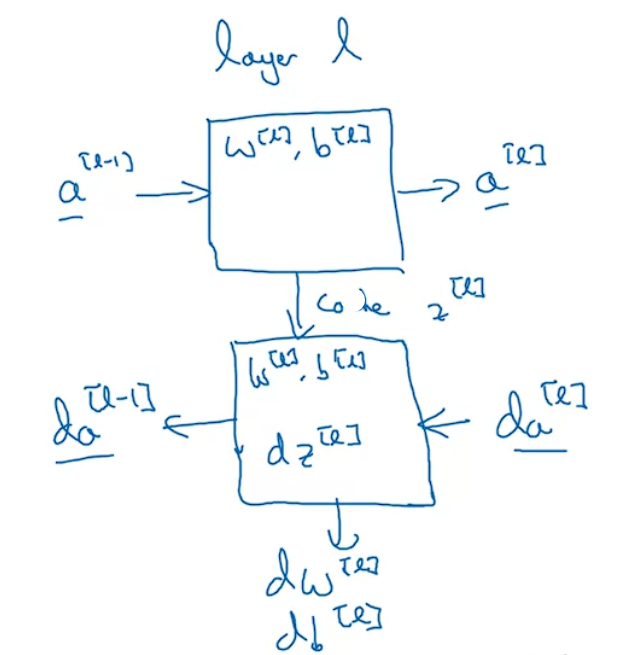
\includegraphics[width=8cm]{12.png}
        \end{figure}
        \item All forward propagation steps will carried out until the hypothesis, $\hat{y}$ is found
        \begin{itemize}
            \item Using cached values, all backpropagation steps will be carried out until $dz^{[1]}$
            \item Parameters $W^{[l]}$ and $b^{[l]}$ can be updated accordingly
            $$W^{[l]}:=W^{[l]}-\alpha dw^{[l]}$$
            $$b^{[l]}:=b^{[l]}-\alpha db^{[l]}$$
        \end{itemize}
        \item Backpropagation will also follow a pattern for all layers in the NN
        \begin{itemize}
            \item $dz^{[l]}=da^{[l]}*g^{[l]'}(z^{[l]})$
            \item $dW^{[l]}=dz^{[l]}a^{[l-1]T}$
            \item $db^{[l]}=dz^{[l]}$
            \item $da^{[l-1]}=W^{[l]T}dz^{[l]}$
        \end{itemize}
        \item For a vectorized implementation:
        \begin{itemize}
            \item $dZ^{[l]}=dA^{[l]}*g^{[l]'}(Z^{[l]})$
            \item $dW^{[l]}=\frac{1}{m}dZ^{[l]}A^{[l-1]T}$
            \item $db^{[l]}=\frac{1}{m}\texttt{np.sum}(dZ^{[l]}\texttt{, axis=1, keepdims=True})$
            \item $dA^{[l-1]}=W^{[l]T}dZ^{[l]}$
        \end{itemize}
    \end{itemize}
    \subsubsection{Parameters vs Hyperparameters}
    \begin{itemize}
        \item Parameters of the NN are the $W$ and $b$ matrices
        \item NN also has a number of associated hyperparameters:
        \begin{itemize}
            \item Learning rate $\alpha$
            \item Number of iterations z`'
            \item Number of layers in the network
            \item Number of hidden units
            \item Choice of activation function
        \end{itemize}
        \item Hyperparameters will control the values of $W$ and $b$
        \item Deep learning has many more hyperparameters than earlier eras of machine learning
        \begin{itemize}
            \item Applying deep learning becomes an empirical process
        \end{itemize}
        \item Intuitions about hyperparameters may be different across different applications
    \end{itemize}
    \end{document}